%auto-ignore
\documentclass{standalone}

\usepackage{graphicx}
\usepackage{tikz}

\begin{document}
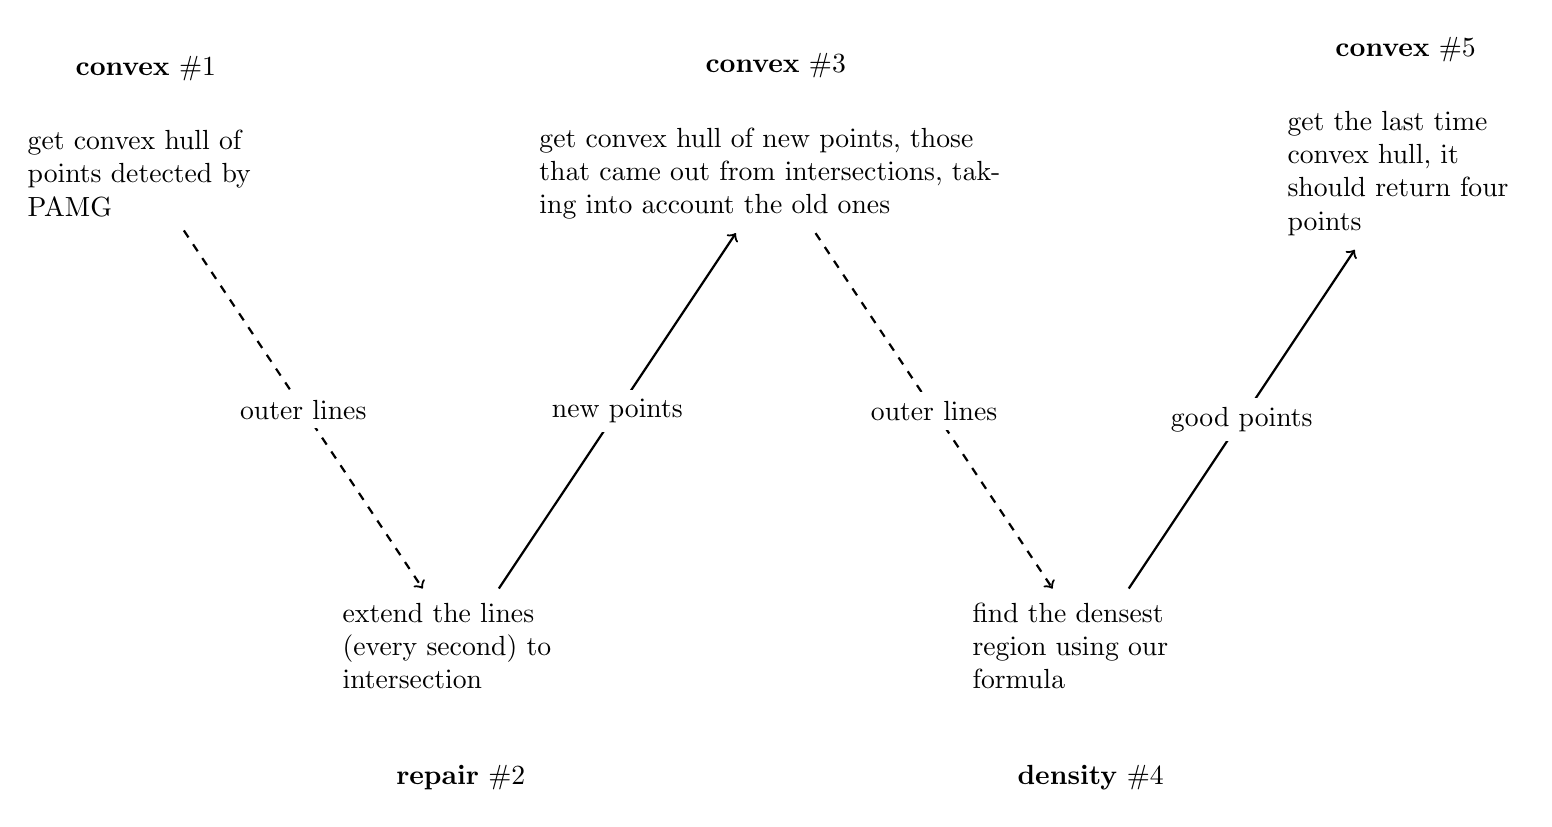
\begin{tikzpicture}
\node[text width=3cm,inner sep=0pt,label={[yshift=0.50cm]\textbf{convex} \#1}] 
(clip1) at (0,6)
	{get convex hull of points detected by PAMG};
\node[text width=3cm,inner sep=0pt,label={[yshift=-2.50cm]\textbf{repair} \#2}]
(clip2) at (4,0) % 0
	{extend the lines (every second) to intersection};
\node[text width=6cm,inner sep=0pt,label={[yshift=0.50cm]\textbf{convex} \#3}]
(clip3) at (8,6)
	{get convex hull of new points, those that came out from intersections, taking
into account the old ones};
\node[text width=3cm,inner sep=0pt,label={[yshift=-2.50cm]\textbf{density} \#4}]
(clip4) at (12,0) % 8
	{find the densest region using our formula};
\node[text width=3cm,inner sep=0pt,label={[yshift=0.50cm]\textbf{convex} \#5}] 
(clip5) at (16,6)
	{get the last time convex hull, it should return four points};
\draw[->,thick,dashed,shorten >=6pt,shorten <=6pt] (clip1) -- (clip2)
	node[midway,fill=white] {outer lines};
\draw[->,thick,shorten >=6pt,shorten <=6pt] (clip2) -- (clip3)
	node[midway,fill=white] {new points};
\draw[->,thick,dashed,shorten >=6pt,shorten <=6pt] (clip3) -- (clip4)
	node[midway,fill=white] {outer lines};
\draw[->,thick,shorten >=6pt,shorten <=6pt] (clip4) -- (clip5)
	node[midway,fill=white] {good points};
\end{tikzpicture}
\end{document}
